First things first, when reading the following chapter, keep one thing in mind: I do my best to design lightweight backpacks, but I wouldn't push it so far as to calling them ultralight packs. There are highly specialised, very talented backpack makers out there who focus all their attention on ultralight hikers (and thru-hikers),  and they come up with amazing featherweight designs. Personally, I have a less drastic approach to weight loss in general, but I am still aiming at a substantial weight reduction without hampering the functionality of my packs.

\subsection{The things one carries, and why it matters}

When you want to have a look at pack weight, you should first consider what exactly you are carrying. For a trip, the weight of my pack is divided in two categories:

\begin{itemize}

	\index{base weight}
	\item My \textbf{base weight} is the weight of my gear, this account for my sleeping system, my clothing, my shelter, and - of course - the pack I carry everything in.

	\index{consumables}
	\item Things like food, water, or the fuel for your stove, are weights which not only vary during a trip, but most importantly will differ from one trip to another. They are the \textbf{consumable} part of the weight you carry.

\end{itemize}

This separation in two categories finds its roots in a very simple truth: although you can be smart about what \textit{consumables} you carry, there is only so much weight you can avoid carrying for your hydration and caloric needs (water can't be altered to weight less, and calories don't come from thin air). Base weight, on the other hand, can be tremendously altered by your choices of items, and how they function together as an ensemble.

If you are reading this, then you probably have done some research already on how to hike lighter, and by now you should be familiar with the big three things which everyone should pay attention to:

\begin{itemize}

	\item Sleeping system
	\item Shelter
	\item Backpack

\end{itemize}

They represent the most part of your base weight, and also are historically the most overlooked piece of equipment when it comes to shaving weight.

\subsection{Example of weight distribution}

If you want to design a backpack, you will need to understand how your gear consumes weight. It is crucial you understand the fine balance between weight and comfort. Every one is different, and will want different levels of comfort, but more so, every trip is different, and will require different pack construction. A simple example can be drawn from a commercial, highly comfortable trekking backpack, which is my go to for loads of 8-10kg, and a frameless, padless backpack I user for loads around 5kg.

This is taken from one of my trips and the following pie chart shows how weight distribution was with conventional gear. I put together this kit to wander the Annapurna Circuit Trek with a focus on \textit{warmth} and \textit{comfort} at high altitude. I had a lot of constrains with the weather as I was hiking for 3 weeks straight, with no expectation for being able to resupply anything other than consumables. In this part of the Himalayas, the altitude variations between 800m and 5400m means temperatures between +25\degree C to -30\degree C.

\def\angle{0}
\def\radius{3}

% Quick pack breakdown Annapurna 2017
% pack      1185   13,72
% photo	    1400   16,21
% sleeping  1530   17,72
% clothing  3230   37,41
% safety    1040   12,05
% walking   249    2,88
% total     8634   100,00

\begin{figure}[H]
\centering

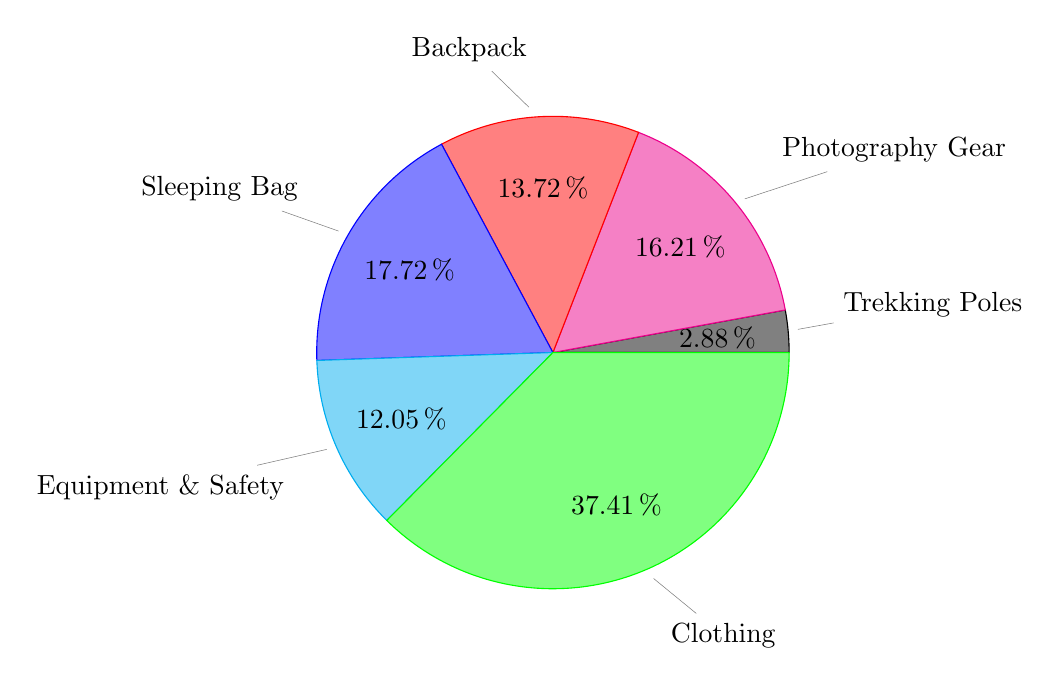
\begin{tikzpicture}
  \foreach \percent/\name/\color in {
      2.88/Trekking Poles/black,
      16.21/Photography Gear/magenta,
      13.72/Backpack/red,
      17.72/Sleeping Bag/blue,
      12.05/Equipment \& Safety/cyan,
      37.41/Clothing/green,
    } {
      \ifx\percent\empty\else % If \percent is empty, do nothing
        \draw[fill={\color!50},draw={\color}] (0,0) -- (\angle:\radius)
          arc (\angle:\angle+\percent*3.6:\radius) -- cycle;
        \node at (\angle+0.5*\percent*3.6:0.7*\radius) {\percent\,\%};
        \node[pin=\angle+0.5*\percent*3.6:\name]
          at (\angle+0.5*\percent*3.6:\radius) {};
        \pgfmathparse{\angle+\percent*3.6}
        \xdef\angle{\pgfmathresult}
      \fi
    };
\end{tikzpicture}

\caption[Example of conventional base weight distribution]{Example of conventional base weight distribution for a 3 weeks backpacking trip with freezing temperatures, but no need for shelter}

\end{figure}


As you can see in this example, the weight of my backpack at the time was competing with my -30\degree celsius down sleeping bag. And I can tell you, both the sleeping bag and the pack where too heavy for what I needed. Despite the fact that my pack was already touching the decently light category at 1.1kg for a very comfortable pack.

An example of shaving a lot of base weight happened in one of my last trip: a fast-paced hike of Scotland's Great Glen Way where I walked 130km in 4 days. For this trip, I had to carry a complete shelter and sleeping system, but not a lot of anything else. So I switched to a custom made ultralight backpack (around 350 grams) and some ultralight 1-person tent (630 grams) with a closed-cell foam sleeping pad (400g). I also used a down quilt instead of a sleeping bag (10\degree C comfort, 395 grams) which was definitely too light.

In should become obvious weight if often a tradeoff with comfort. In that regard, every being different, you will have to find your "sweet spot" on your own.

\begin{table}[H]
  \centering
  \begin{tabular}{ | l | p{3cm} | p{3cm} | }
    \hline			
    \textbf{Item} & \textbf{Himalayas} & \textbf{Scotland} \\
    \hline
    Approx. Base Weight & 9kg & 6.5kg \\
    \hline
    Days on the trail & 20 & 4 \\
    \hline
    Backpack & 1.1kg & 350 grams \\
    \hline
    Sleeping system & 1.5kg \newline (bag only) & 1.4kg \newline (full shelter) \\
    \hline
    Trekking Poles & 250 grams & N/A \\
    \hline
  \end{tabular}
  \caption{Base weight diet}
\end{table}

\subsection{Weight categories \& purpose}

The purpose of a pack is obviously to carry things. But the way I will use it make a huge difference in the way I design a pack. For example, I care little for inside pockets, I always carry some stuff outside my pack, I usually lug around loads between 3 to 8 kilograms (depending on how long I'm hiking for, and in which conditions) but most of my gear compresses well, so 40 litres is usually good enough.
For loads equivalent to 40 litres weighing 7 to 9kilograms, most commercially available backpacks oscillate between 1.20 and 1.80 kilograms, and specialised ultralight backpacks can go down to 300 grams.
